
\subsubsection{DCT Transform}
DCT transformation like fourier transform, intends to reduce existed redundancy in the frequency domain. The equations of two dimensional discrete cosines transform (DCT), And inverse discrete cosine transform (IDCT), are given below in order.
\begin{align}
    F(u,v) &= \sqrt{\frac{2}{MN}}C(u)C(v)\sum_{x=0}^{M-1}\sum_{y=1}^{N-1}f(x,y)cos[\frac{\pi}{2N}(2x+1)u]cos[\frac{\pi}{2M}(2(y+1)v)] \\
    f(u,v) &= \sqrt{\frac{2}{MN}}\sum_{x=0}^{M-1}\sum_{y=1}^{N-1}C(u)C(v) F(x,y)cos[\frac{\pi}{2N}(2x+1)u]cos[\frac{\pi}{2M}(2(y+1)v)]
\end{align}
where $M$ and $N$ are sizes of the image. And 
\begin{align}
    C(u) = \begin{cases}
    \frac{1}{\sqrt{2}}, \quad u=0;\\
    1, u=1,2,...N-1;
    \end{cases}
\end{align}

\begin{figure}[!htbp]
\centering
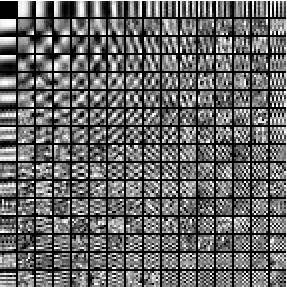
\includegraphics[width=0.2\linewidth]{images/DCT_dict.png}
\caption{A standard discrete cosine (DCT) dictionary;}
\label{dic1}
\end{figure}

\begin{algorithm}[!htbp] 
\caption{Block-sparse Dictionary Update}
\label{alg:Framwork} 
\begin{algorithmic}
\REQUIRE ~~\\%Input
The input signal $\mathbf{Y}$, block sparsity level $k$, and maximal block size $s$.\\
\ENSURE ~~\\ %Output
Learned Dictionary $\mathbf{\Phi}$ with optimal block struture $d$.\\
% --------------------------------------------------------\\
\STATE 1. Initialise the dictionary $D(0)$ as the outcome of K-SVD.\\
\STATE 2. For $N$ number of iterations.\\
\STATE \quad - Fix dictionary $\mathbf{\Phi}^{(m-1)}$ and update coefficients $x^{m}$ and block structure $d^{(m)}$ by applying sparse agglomerative clustering.\\
\STATE \quad - Fix the block structure $d^(m)$ and update the dictionary atoms $\mathbf{\Phi}^{(m)}$ by applying BS-SVD.\\
\end{algorithmic}
\end{algorithm}

According to whether the original cover image and watermark is needed or not during the extraction process, digital watermarking techniques can be divided in to three catagories: non-blind, semi-blind to blind digital watermarking techniques\cite{Yu2017}. We focus on blind techniques which does not need the original images but only a security 'key' for decoding the watermark.\\

\subsection{MCA applied to Digital Image Watermarking}
Apart from using \textit{Independent Component Analysis} as an blind signal separation (BSS) tool, We can also treat it as a statistical model for feature extraction. The fundamentals of independence and sparseness lead to the representations and interpretation which exhibit remarkable similarity to human perception in different images \cite{BELL19973327}. Therefore, we can deduct that ICA
models can perform well in image processing tasks acquiring features related to human perceptions. Based on that ideas, an approach using ICA is proposed in \cite{inproceedingsICA_watermark}. It is classified in the transformed domain method as the watermarking is inserted in the image after it has been projected into the ICA space. \\

Now we explain the ICA watermark method introduced in \cite{inproceedingsICA_watermark}. It is worth noting that the original algorithm could only be applied to watermark which has the same size as cover image. We are able to extend it to a more general usage scenario where a smaller watermark can be inserted. We first address the problem of feature learning, inserting the watermark and then watermark extraction.

\begin{figure}[H]
\centering
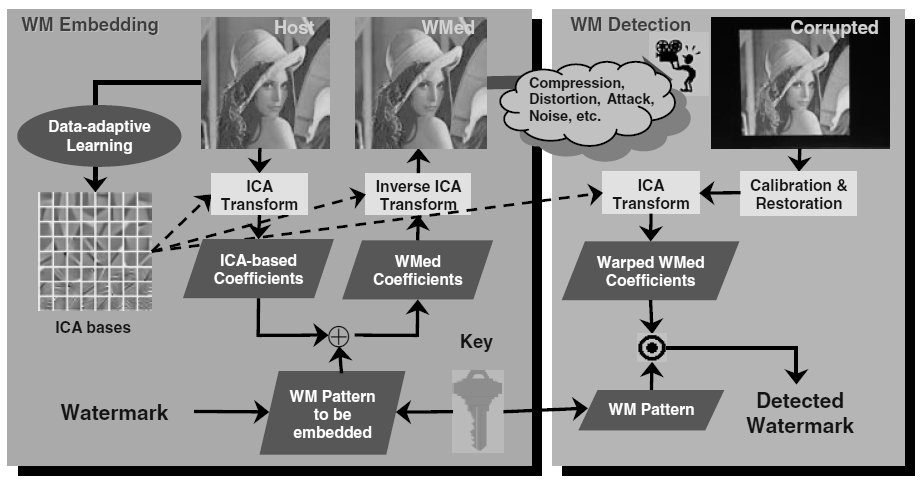
\includegraphics[width=0.8\textwidth]{images/ICA_flowchart_gray.png}
\caption{The flowchart of the whole ICA-based watermarking scheme. \cite{LuWei_ICA}}
\label{flow_ICA}
\end{figure}

\subsubsection{ICA feature learning}
hadamard code\\
Suppose we have a cover image of size $n\times m$ and a watermark image of size $k\times l$ The cover image matrix is divided into smaller blocks $C_{p,q}(i,j)$ with indexes
\begin{align}
    i,j &= 1,2,...,k\\
    p &= 1,2,...,\floor{\frac{n}{k}}\\ 
    q &= 2,3,...,\floor{\frac{m}{l}} 
\end{align}

And $C_{p,q}(i,j)$ is defined as patches of the cover image.

\begin{align}
    C_{p,q}(i,j) = I(k(p-1)+i, k(q-1)+j)
\end{align}
By applying ICA to blocks $C_{p,q}$, we then preserve only the $r$ independent components with larger variance (energy) ant it restores the image starting from these $r$ components. This is because ICA method could decompose the image into a set of basis functions to build a group of images. Suppose the watermark image has size $k \times l$ for convenience, we can now apply the same feature extraction routine to the watermark image.

\subsection{Performance measures}
\subsubsection{PSNR}
In order to make quantitative analysis of the digital watermark insertion/extraction process in experiments, the\textit{ Peak Signal to Noise Ratio} (PSNR) index is calculated to assess the effect from gray-level fidelity aspect. The definitaion of PSNR is as follows.
\begin{equation}
    \text{PSNR}(\mathbf{x,y}) = 10log_{10}\frac{(MAX_I)^2}{MSE(\mathbf{x,y})} 
\end{equation}
where $MAX_I$ is the maximum possible pixel value of image \mathbf{x} and image \mathbf{y}. Because we use mono-color gray scale image as the cover image and watermark. The value of $MAX_I$ is 255. $MSE(\mathbf{x,y})$ represents the Mean Square Error between the original watermark and extracted watermark, and it is calculated as follows.
\begin{equation}
    MSE(\mathbf{x,y}) =  \frac{1}{mn}\sum_{i=0}^{m-1}_{j=0}^{n-1}[\mathbf{x}(i,j) - \mathbf{y}(i,j)]^2
\end{equation}
where $m$ and $n$ are the dimension of image $\mathbf{x}$ and image $\mathbf{y}$. PSNR can evaluate both the inserted cover image quality and the extracted watermark quaility. When measuring the cover image, the larger the PSNR value means less discrepancies exists between the original image and the altered one, hence better imperceptibility. When PSNR measures the watermark, larger value yields better extracting quality.

\subsubsection{Normalised Correlation}
Normalised correlation (NC) measures the similarity between the recovered watermark and original watermark. The larger its value, the less defects it is in the recovered data, and the method is more robust against attacks.

\begin{equation}
    NC =  \frac{\sum_{i=0}^{m-1} \sum_{j=0}^{n-1}W(i,j) W'(i,j)} {\sum_{i=0}^{m-1} \sum_{j=0}^{n-1} W^2(i,j)}
\end{equation}

\subsubsection{Insertion}
By applying ICA algorithm to the cover image, we obtain the demixing matrix $\mathbf{B}^I$ and independent ICA components (basis) $\mathbf{y}^I_t$. 
We propoes to replace the r components from $\mathbf{y}^I_t$ with first $k^2 -r$ components of the watermark image $\mathbf{y}^W_t$, yields the watermarked image  $\mathbf{y}^V_t$. Multiplying the inverse of $\mathbf{B}^I$ with $\mathbf{y}^V_t$ gives the watermarked image in human vision. 

\begin{align}
    \mathbf{y}^V(h) &=  \mathbf{y}^I(h) \quad h = 1,...,k^2-r \\
    \mathbf{y}^V(k^2-h+1) &= \alpha  \mathbf{y}^W(h) \quad h = 1,...,r
\end{align}
where $\alpha$ defines the intensity (perception) of the watermark. However the insertion method is not unique. 
There is is a trade off between imperceptibility and robustness. 
our method of inserting the watermark in sorted basis with high energy results in good imperceptibility and moderate robustness.
we should avoid modulating coefficients that have less energy, because they are the least robust components under watermark attacks. More discussion can be found in \cite{LuWei_ICA} and \cite{Yu2017}.

\subsubsection{Extraction}
First we repeat steps in insertion section and divide the watermarked image into patches $\mathbf{x}_t$ again. Then we obtain the ICA components by imposing the demixing matrix calculated in Insertion step. Note that the demixing matrix $\mathbf{B}^I$is also the key throughout the whole process.

\begin{align}
    \mathbf{y}^V(h)  &=  \mathbf{B}^I\mathbf{x}_t^v \\
    \mathbf{y}_t^W(h) &= \mathbf{y}^V(k^2-h+1) \quad h = 1,...,r
    \label{eq38}
\end{align}
Finally we extract and reshape the watermark signal refer to Equ.\ref{eq38}. 

The earliest method is referred as techniques in least significant bits (LSBs), where watermark image does not affect much the final quality of image due to its insignificant location for embedding. The method possesses minimum embedding capacity and meanwhile is apt for destroying as most easy as possible.

One of the major limitation of this kind of methods is that they are seldom based on Human Vision System (HVS) that may be regarded as the final judge for a successful watermarking technique \cite{LuWei_ICA}. Comparison between embedded watermark images using different techniques in the next section reveals the relatively poorer imperceptibility of DCT methods.


\begin{figure}[H]
\centering
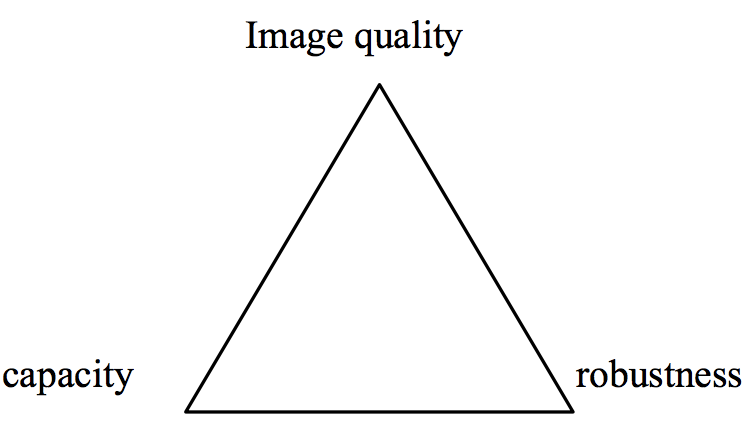
\includegraphics[width=0.4\textwidth]{images/watermark_tradeoff.png}
\caption{ three important parameters in watermarking systems}
\label{trade-off}
\end{figure}
In order to improve any parameter in the triangle, there
must be a trade-off \cite{DCT_watermark}. 

This chapter has considered the BSS methods which will be used in next stage of this project. Firstly, the linear instantaneous model was introduced and BSS assumptions were stated. We then introduced performance metrics to evaluate the performances of various BSS algorithms. The problem was then extended to the case of sparsity where morphological component analysis is discussed. 